\documentclass[10pt]{article}
\usepackage{a4wide}
\usepackage[english]{babel}
\usepackage{graphicx}
\usepackage{tabu}
\usepackage{textcomp}
\usepackage{fancyhdr}
\usepackage{lastpage}
\usepackage{titlesec}
\usepackage{lscape}
\usepackage{longtable}
\usepackage{color}
\usepackage{listings}
\usepackage{xkeyval}
\usepackage{hyperref}

\definecolor{mygreen}{rgb}{0,0.6,0}
\definecolor{mygray}{rgb}{0.5,0.5,0.5}
\definecolor{mymauve}{rgb}{0.58,0,0.82}

\lstset{ % Syntax highliughting for java
    backgroundcolor=\color{white},   % choose the background color; you must add \usepackage{color} or \usepackage{xcolor}
    basicstyle=\footnotesize,        % the size of the fonts that are used for the code
    breakatwhitespace=false,         % sets if automatic breaks should only happen at whitespace
    breaklines=true,                 % sets automatic line breaking
    captionpos=b,                    % sets the caption-position to bottom
    commentstyle=\color{mygreen},    % comment style
    deletekeywords={...},            % if you want to delete keywords from the given language
    escapeinside={\%*}{*)},          % if you want to add LaTeX within your code
    extendedchars=true,              % lets you use non-ASCII characters; for 8-bits encodings only, does not work with UTF-8
    frame=none,                    % adds a frame around the code
    keepspaces=true,                 % keeps spaces in text, useful for keeping indentation of code (possibly needs columns=flexible)
    keywordstyle=\color{blue},       % keyword style
    language=Octave,                 % the language of the code
    morekeywords={*,...},            % if you want to add more keywords to the set
    numbers=left,                    % where to put the line-numbers; possible values are (none, left, right)
    numbersep=5pt,                   % how far the line-numbers are from the code
    numberstyle=\tiny\color{mygray}, % the style that is used for the line-numbers
    rulecolor=\color{black},         % if not set, the frame-color may be changed on line-breaks within not-black text (e.g. comments (green here))
    showspaces=false,                % show spaces everywhere adding particular underscores; it overrides 'showstringspaces'
    showstringspaces=false,          % underline spaces within strings only
    showtabs=false,                  % show tabs within strings adding particular underscores
    stepnumber=5,                    % the step between two line-numbers. If it's 1, each line will be numbered
    stringstyle=\color{mymauve},     % string literal style
    tabsize=4,                       % sets default tabsize to 2 spaces
    title=\lstname                   % show the filename of files included with \lstinputlisting; also try caption instead of title
}
%%%%%%
%% Variables for version and release status
%% useage: \version
%%%%%%
\newcommand\module{CS22510}
\newcommand\moduleName{C++, C and Java Programming Paradigms}
\newcommand\authorText{Nicholas Dart}
\newcommand\authorUsername{nid21}
\newcommand\studentID{130057750}
\newcommand\assesser{Dr Frederic Labrosse, Dr Neal Snooke}

%%%%%%
%% Alias
%%%%%%
%\newcommand{\sectionbreak}{\clearpage}    %% Allways start a section on a new page

\title{ \huge \module Assignment \\ \Large \moduleName}
\author{
    \vspace{100pt}
    \begin{tabular}{ r || l }
        Author          & \authorText (\authorUsername)\\
                        & \studentID \\
        Date Published  & \today \\
                        & \\
        Assessed By     & \assesser \\
        Department      & Computer Science \\
        Address         & Aberystwyth University \\
                        & Penglais Campas \\
                        & Ceredigion \\
                        & SY23 3DB \\
    \end{tabular} \\
    Copyright \textcopyright Aberystwyth University 2015
    %get rid of the date on the titlepage
    \date{}
}

\pagestyle{fancy}
\fancyhf{}
\lhead{\module~Assignment}
\rhead{\authorText~-~\studentID}
\rfoot{Page \thepage \hspace{1pt} of \pageref{LastPage}}
\lfoot{Aberystwyth University - Computer Science}

\begin{document}
    \setcounter{page}{1}

    \maketitle
    \thispagestyle{empty}
    \clearpage

    \section{Design}
        I designed the rough solution to this coursework together with another student, Owen Garland. Together we outlined the required features and came up with a loose class diagram for how we expect classes and objects to interact. This is shown below:

        \begin{figure}[bh]
            \centering
            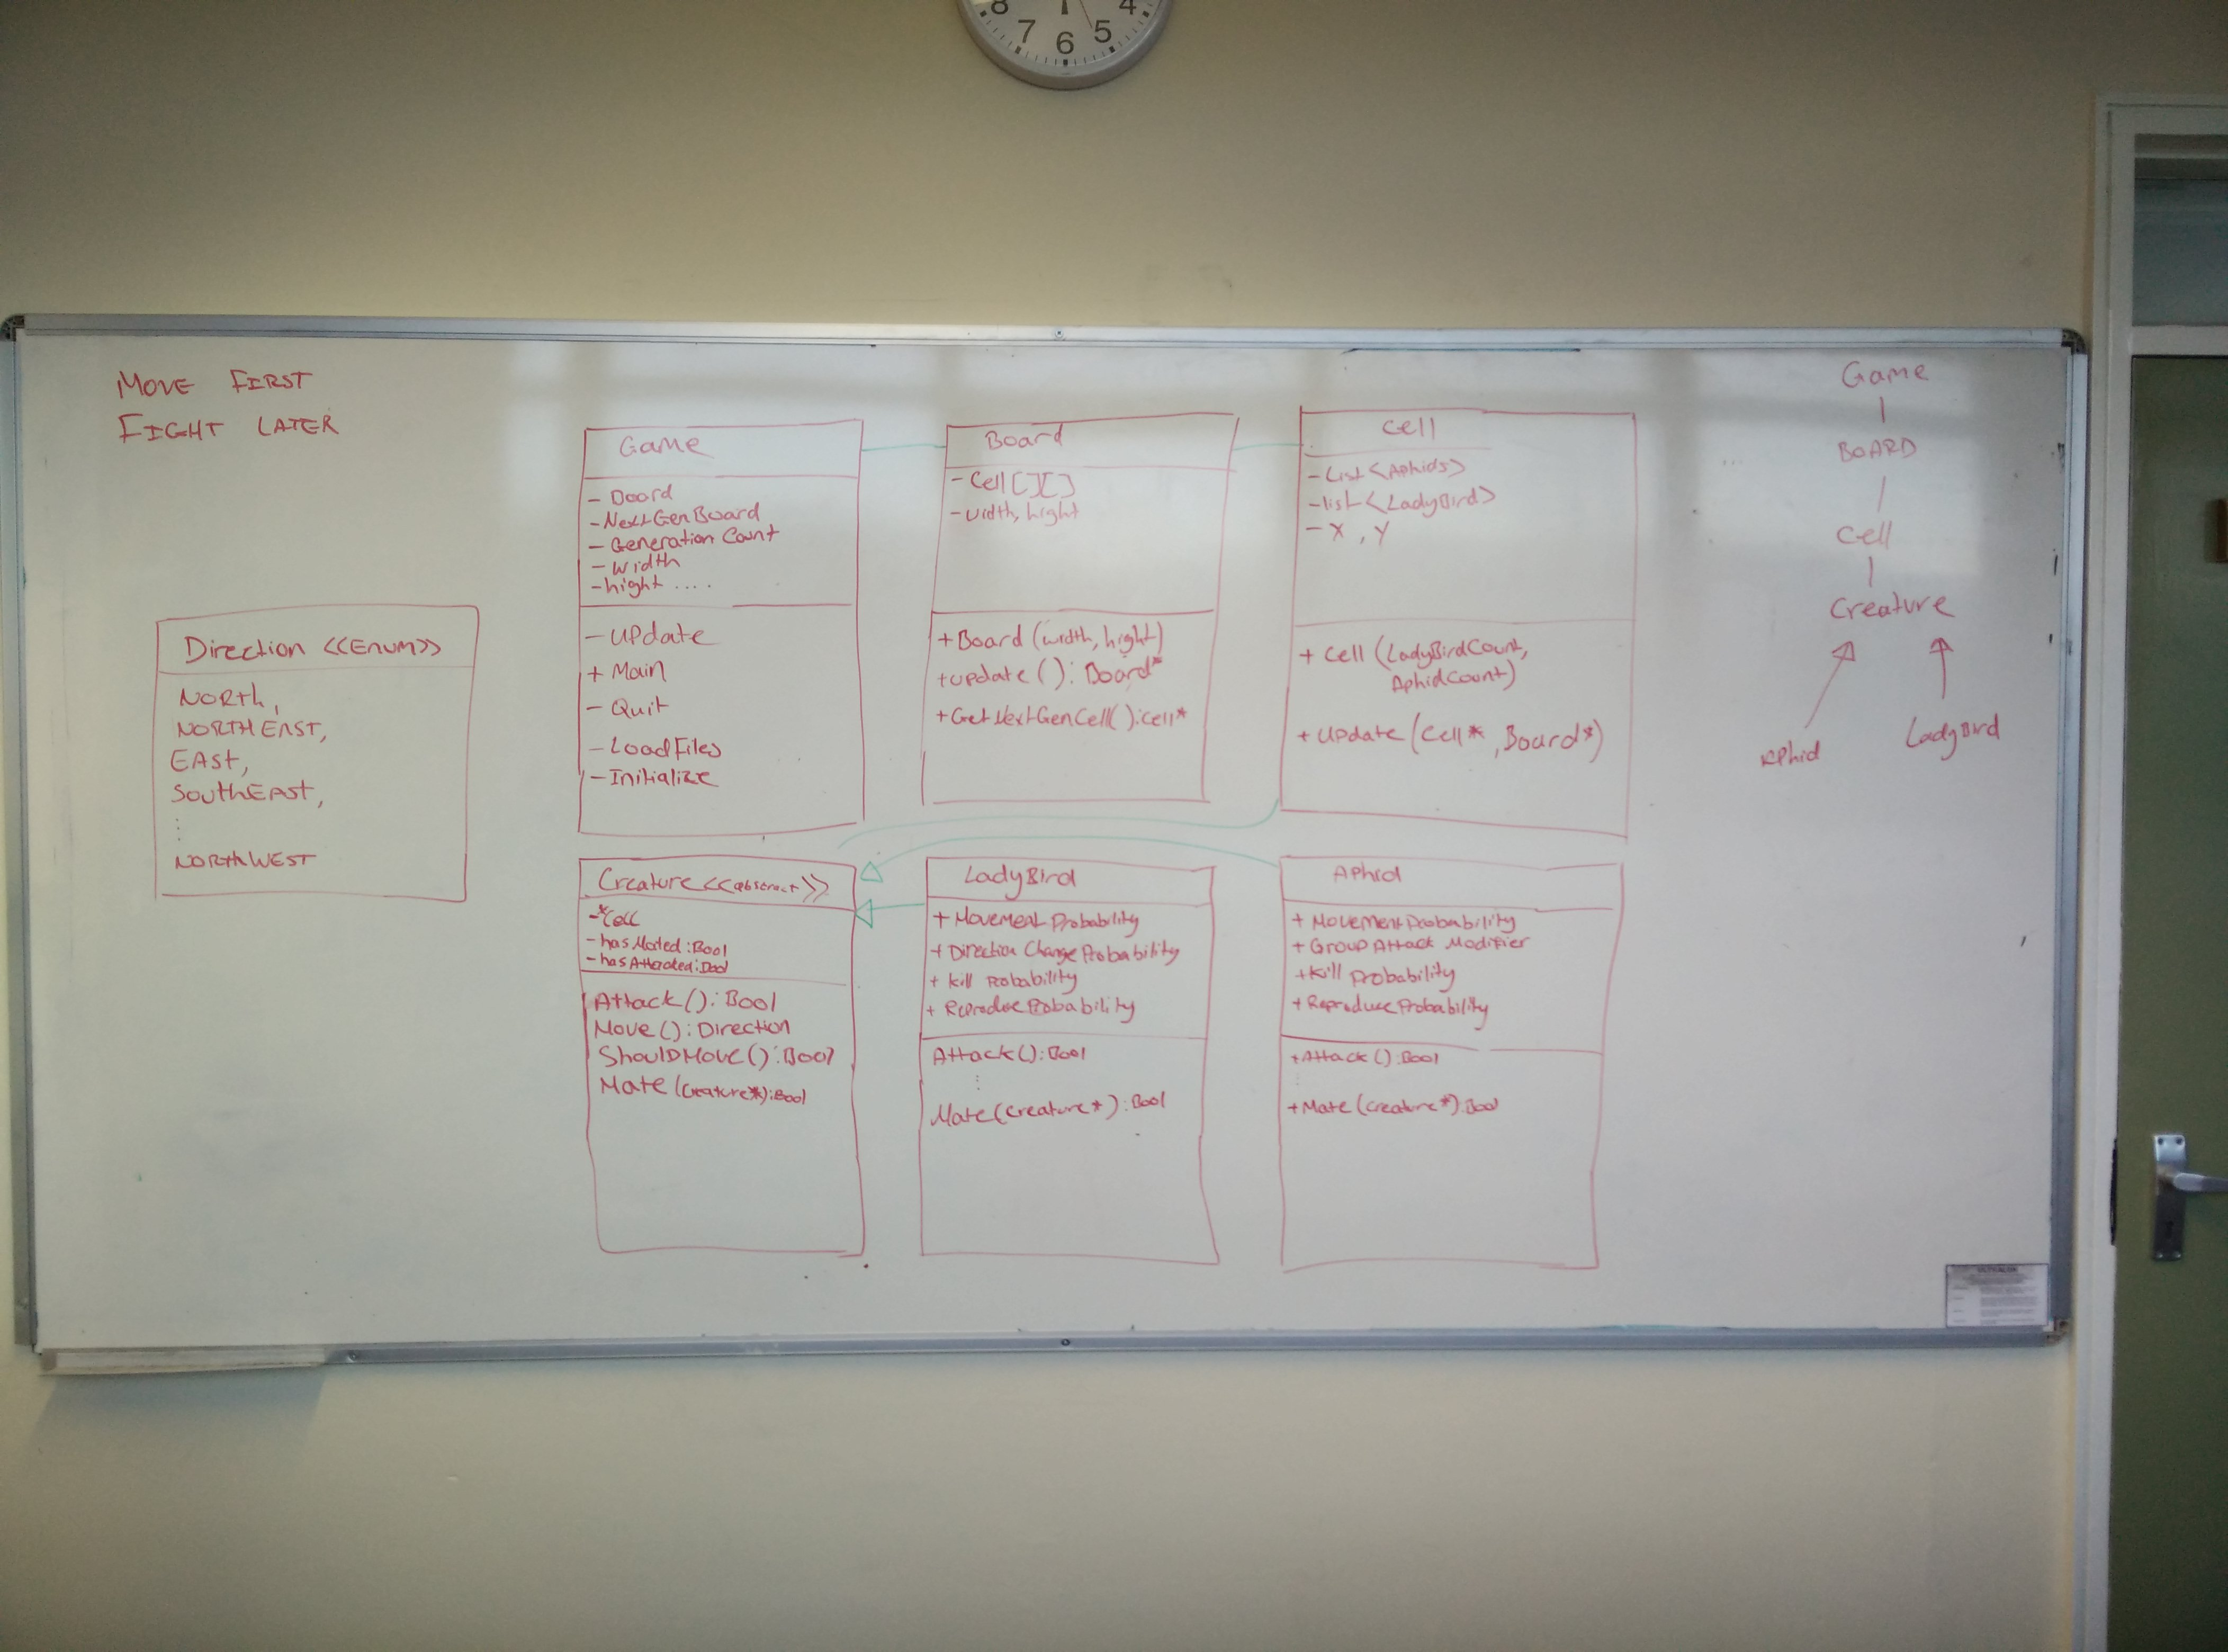
\includegraphics[scale=0.1]{roughPlan.jpg}
            \caption{Full image included named ``roughPlan.jpg''}
        \end{figure}

        This was then the starting point for my implementation, however we uncovered several vague definitions or scenario in which the outcome is undefined. These we decide not to agree on a solution to as not to plagiarise each others work. They are as follows;

        \begin{itemize}
            \item When a creature gets killed, can it continue it's work for this generation?
            \item Do ladybirds have a preferred starting direction or a random one?
            \item If an aphid attacks, will all it's brethren in the cell automatically attack, or is it then up to them to help?
            \item Can a creature be killed in the same generation as it's born?
        \end{itemize}

    \section{Implementation}
        The implementation largely followed the design above, however the outcome was not as object orientated as I feel I would have been able to achieve in Java. Several areas, including adding and storing creatures are not as generic as I would like; I am storing aphids and ladybirds separately, not as generic creatures. This was due to the fact a ladybird or aphid has to know what type the creature it is interacting with is. As such things like movement of the board (which does not care about surroundings except being off the board) are less elegant and require two loops, one for aphids and one for creatures.

        I also feel (and \#c++ on irc.freenode.net agree) that my use of pointers was excessive and not necessary. I have tried to redactor my work to reduce this, however there still remains a large number of probably unnecessary pointers. I did however change from using an array of cells defined as \texttt{Cell ***cells}, however this was changed to a \texttt{vector<vector<Cell>> Cells} as described in \url{http://www-h.eng.cam.ac.uk/help/tpl/languages/C++/vectormemory.html}.

        I also started out using \texttt{std::list} however I also changed these to lists, again under recommendations from people on irc.

    \section{Additional Features}
        I implemented a seed feature to the game, where if a given seed and input files are consistent across ``games'' then the outcome of the senario will be the same, this was achieved simply by allowing the user to enter a seed or if not, using the current date time as the seed. The game will also terminate when either side has won.

        \begin{figure}[bh]
            \centering
            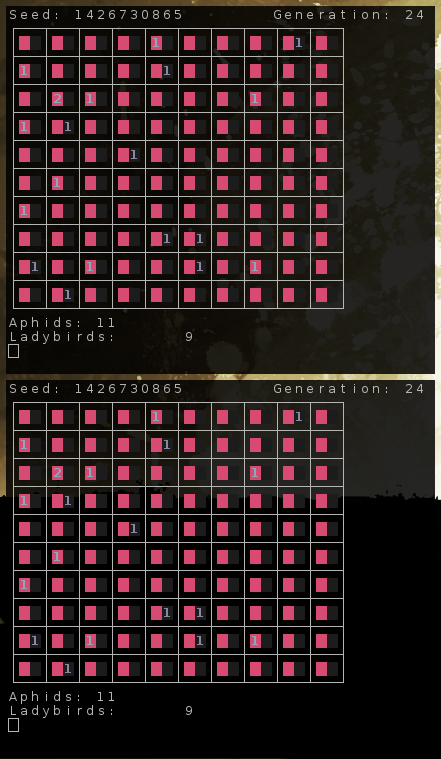
\includegraphics[scale=0.5]{sameSeeds.png}
            \caption{An example with two games of the same seed and input files}
        \end{figure}
 

\end{document}